\section{Streaming Clustering and Coreset Trees}
\label{sec:background}
To provide context for how algorithms in this paper will be used, we describe a
generic ``driver'' algorithm for streaming clustering.  We also discuss the
coreset tree (\ct) algorithm.  This is both an example of how the driver works
with a specific implementation and a quick review of an algorithm from prior
work that our algorithms build upon.

%----------------------------
\begin{algorithm}[tb]
\caption{Stream Clustering Driver}\label{algo:cluster-init}
\label{algo:cluster-update}
\label{algo:cluster-query}
\fnDef{$\clusterupdate(\object, p)$}{
  \tcp{Insert new point $p$ from the stream into $\object$}
  Add $p$ to $\object.C$\;
  
  \If{$(|\object.C| = m)$}
  {
    $\object.\mathcal{D}$.Update($\object.C$)\;
    $\object.C \gets \emptyset$\;
  }
}
\fnDef{$\clusterquery()$}{
  $C_1 \gets \object.\mathcal{D}.Coreset()$\;
  \Return $\kmpp(k, C_1 \cup \object.C)$\;
}
\end{algorithm}
%------------------------------

\subsection{Driver Algorithm}
The ``driver'' algorithm (presented in Algorithm~\ref{algo:cluster-update}) internally keeps state as an object $\object$. The state $\object$ involves a specific implementation of a clustering data structure $\mathcal{D}$ and an auxiliary point set $C$. The point set $C$ receives every new point from the stream and with maximum capacity $m$. The size $m$ is the coreset size where the value is determined by the coreset construction algorithm. Once the size of $C$ increases to $m$, the $m$ points will be inserted into the clustering data structure $\mathcal{D}$, as well $C$ will be emptied.  So $C$ groups arriving points into batches at the granularity of size $m$ and stores the current batch.  Subsequent algorithms in this paper, including \ct, are implementations for the clustering data structure $\mathcal{D}$.

%------------------------------------------------------------------------------
\subsection{\ct: $r$-way Merging Coreset Tree}
\label{sec:cstree}
%------------------------------------------------------------------------------

\newcommand*{\qtree}[0]{\ensuremath{Q}\xspace}
%------------------------------------------------------------------------------
The \emph{$r$-way coreset tree} (\ct{}) turns a traditional batch algorithm for
coreset construction into a streaming algorithm that works in limited space.
Although the basic ideas are the same, our description of \ct{} generalizes the
coreset tree of Ackermann et~al.~\cite{AMR+12}, which is the special case when
$r = 2$.


\remove{
%--------------------
\begin{figure*}[tb]
  \centering
  \includegraphics[width=.99\textwidth]{figs/coreset-tree-smaller-examples}
%  \centering
%  \includegraphics[width=.96\columnwidth]{figs/coreset-tree-illus}
  \caption{Illustration of a coreset tree with $r = 3$.}
\label{fig:ct-example}
\end{figure*}
%--------------------
}

\noindent\textbf{The Coreset Tree:}
A coreset tree $\qtree$ maintains \emph{buckets} at multiple levels.  The
buckets at level $0$ are called \emph{base buckets}, which contain the original
input points.  The size of each base bucket is specified by a parameter $m$.
Each bucket above that is a coreset summarizing a segment of the stream observed
so far.  In an $r$-way \ct, level $\ell$ has between $0$ and $r-1$ (inclusive)
buckets, each is a summary of $r^\ell$ base buckets.

Initially, the coreset tree is empty. After observing $n$ points in the stream,
there will be $N = \lfloor n/m \rfloor$ base buckets (level 0). Some of these
base buckets may have been merged into higher-level buckets.  The distribution
of buckets across levels obeys the following invariant:
\begin{quote}
  If $N$ is written in base $r$ as $N = (s_q, s_{q-1}, \dots, s_1, s_0)_r$, with
  $s_q$ being the most significant digit (i.e., $N = \sum_{i=0}^q s_ir^i$), then
  \emph{there are exactly $s_i$ buckets in level $i$}.
\end{quote}


%An example is given in Figure~\ref{fig:ct-example}A: Having observed $N = 8$
%base buckets worth of data, the coreset contains $2$ buckets at level $0$, $2$
%buckets at level $1$, and none above this level, corresponding to
%$N = 8 = (2,2)_3$ in base $3$.


%--------------------
\begin{algorithm}[t]
\caption{Coreset Tree Algorithm}\label{algo:ctfunctions}
\label{algo:ctinit}
\label{algo:ctupdate}
\label{algo:ctquery}
% \fnDef{$\ctinit(r, k, \eps)$}{
%   $Q \gets \emptyset $\;
%   Remember parameters $r$, $k$, and $\eps$.
% }
\tcp{\emph{Input:} bucket $b$}
\fnDef{$\ctupdate(b)$}{
  Append $b$ to $Q_0$\;
  $j \gets 0$\;
  \While{$|Q_j| \ge r$} {
    $U \gets \coreset(k, \eps, \cup_{B \in Q_j} B)$\;
    Append $U$ to $Q_{j+1}$\;
    $Q_j \gets \emptyset $\;
    $j \gets j+1$ \;
  }
}
\tcp{For query method $\clusterquery()$}
\fnDef{\ctcoreset()}{
  \Return{$\bigcup_{j} \{\bigcup_{B \in Q_j} B \}$}\;
}
\end{algorithm}
%--------------------


\noindent{}\emph{\textbf{How is a base bucket added?}}
The process to add a base bucket is reminiscent of incrementing a base-$r$
counter by one, where merging is the equivalent of transferring the carry from
one column to the next.  More specifically, \ct maintains a sequence of
sequences $\{Q_j\}$, where $Q_j$ is the buckets at level $j$. To incorporate a
new bucket into the coreset tree, \ctupdate{}, presented in
Algorithm~\ref{algo:ctupdate}, first adds it at level $0$. When the number of
buckets at any level $i$ of the tree reaches $r$, these buckets are merged,
using the coreset algorithm, to form a single bucket at level $(i+1)$, and the
process is repeated until there are fewer than $r$ buckets at all levels of the
tree. An example of how the coreset tree evolves after the addition of base buckets 
is shown in Figure~\ref{fig:coreset-tree}.

%---------------
\begin{figure}
  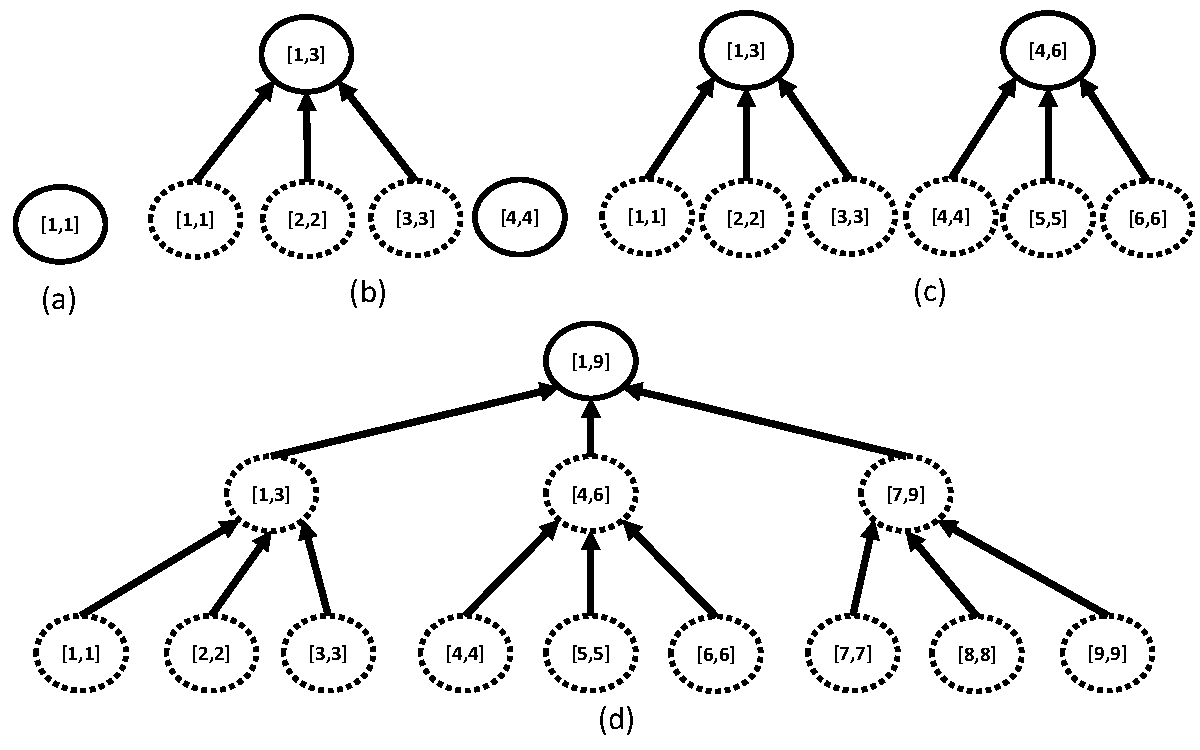
\includegraphics[width=0.5\textwidth, height=7cm]{figs/coreset-tree.pdf}
  \caption{Illustration of a $3$-way coreset tree (\ct), showing the states after receiving number of base buckets 
  (a) $1$, (b) $4$, (c) $6$, (d) $9$. The notation $[l,r]$ denotes a coreset of all points in buckets number from $l$ to $r$, both endpoints inclusive. The coreset tree consists of coresets represented by ellipses, each is a base bucket (level $0$) or has been formed by merging multiple coresets from lower levels. A coreset becomes inactive when it is merged and represented by a dotted bordered ellipse.}
\label{fig:coreset-tree}
\end{figure}
%---------------

%Fig.~\ref{fig:ct-example}B--D demonstrate steps of this process. There was
%previously $N=8$ in Fig.~\ref{fig:ct-example}A.  To add one base bucket, the
%bucket is first added to level 0 (Fig.~\ref{fig:ct-example}B), causing level $0$
%to be full and triggering level-$0$ buckets to be merged into level $1$
%(Fig.~\ref{fig:ct-example}C). But then, level 1 also becomes full, so the
%level-$1$ buckets are merged into level $2$ (Fig.~\ref{fig:ct-example}D).


% %\medskip
% \noindent\textbf{Coreset Tree Maintenance:} 
% %
% The coreset tree maintains the buckets as a list of lists.  
% Algorithm~\ref{algo:ctfunctions} contains detailed descriptions of how to maintain
% the coreset tree structure.  The high-level ideas are as follows: Let $\qtree_j$
% denote the list of buckets at level $j$.  Initially, \ctinit{} is called, which
% creates an empty list.  The stream clustering driver accumulates input points
% and calls \ctupdate{} when a base bucket is full.  To incorporate a new bucket
% into the coreset tree, \ctupdate{} adds it at level $0$.  When the number of
% buckets at any level $i$ of the tree reaches $r$, these buckets are merged to
% form a single bucket at level $(i+1)$, and the process is repeated until there
% are fewer than $r$ buckets at all levels of the tree.  This process is
% reminiscent of incrementing a base-$r$ counter by one, where merging is the
% equivalent of transferring the carry from one column to the next.

%As an example, Figures~\ref{fig:ct-example}B and C show the result of adding one
%base bucket to $N = 19$, and then to $N = 20$, which triggers a merge of three
%level-$0$ buckets into one level-$1$ bucket.

\noindent{}\emph{\textbf{How to answer a query?}}  The algorithm simply unions all the active buckets together, specifically
$\bigcup_{j} \{\bigcup_{B \in Q_j} B \}$.  Notice that the driver will combine
this with a partial base bucket before deriving the $k$-means centers.

Following lemmas stating the properties of the \ct algorithm. We use the following definition in proving clustering guarantees.
%---------------------
\begin{definition}[Level-$\ell$ Coreset]
  For $\ell \in \Z_{\geq 0}$, \emph{a $(k,\eps, \ell)$-coreset} of a point set
  $P \subseteq \R^d$, denoted by $\coreset(k, \eps, \ell, P)$, is as follows:
The level-$0$ coreset of $P$ is $P$. % (i.e., $\coreset(k,\eps, 0, P) = P$).
For $\ell > 0$, a level-$\ell$ coreset of $P$ is a coreset of the union
of $C_i$'s (i.e., $\coreset(k, \eps, \cup_{i=1}^t C_i)$), where each
$C_i$ is a level-$\ell_i$ coreset, $\ell_i < \ell$, of $P_i$ such that
$\{P_j\}_{j=1}^t$ forms a partition of $P$.
\end{definition}
%---------------------

%---------------------
\begin{lemma}
\label{lemma:cstree-level2}
For a point set $P$, parameter $\eps > 0$ and integer $\ell \ge 0$, 
if $C = \coreset(k,\eps,\ell,P)$ is a level $\ell$-coreset of $P$, 
then $C = \coreset(k, \eps', P)$ where $\eps' = \left(1+\eps \right)^{\ell} - 1$.
\end{lemma}
\begin{proof}
	We prove this by induction, denote our lemma as proposition $\mathcal{P}$. 
	Consider the base case $\ell = 0$, by definition,
	the level $0$ coreset is in the base buckets where original input points inside, 
	and $\left(1+\epsilon \right)^{0} - 1 = 0$.
	
	Now consider level $\ell > 0$. Suppose that $\mathcal{P}(L - 1)$ is true, 
	the task is to prove ${\cal P}(L)$.
	Suppose $C$ is a level $L$ coreset, then $C$ is merged by $r$ level $(L - 1)$ coresets. 
	For $i=1 \ldots r$, let $C_i$ denote the level $(L - 1)$ coreset, 
	each summarizing a point set $P_i$. 
	Then $C$ must be of the form $C = \coreset(k, \epsilon, \cup_{i=1}^r C_i)$.

	By the inductive hypothesis, we know that $C_i = \coreset(k, \epsilon_i, P_i)$
	where $\epsilon_i = \left(1 + \epsilon \right)^{L-1} - 1$.  
	Let $C' = \cup_{i=1}^r C_i$. From Observation~\ref{obs:coreset1} and using
	$P = \cup_{i=1}^r P_i$, it must be true that $C'= \coreset(k, \epsilon_i, P_i)$.
	Since $C = \coreset(k, \epsilon, C')$ and using Observation~\ref{obs:coreset2}, we
	get $C=\coreset(k, \gamma, P)$ where
	$\gamma = (1 + \epsilon)(1 + \epsilon_i) - 1$. Simplifying, we get
	$\gamma = (1 + \epsilon)(1 + \left(1 + \epsilon \right)^{(L-1)} - 1)-1 =
	\left(1 + \epsilon \right )^L - 1$.
	This proves the inductive case, which completes the proof.
\end{proof}
%--------------------------


\begin{fact}
\label{fact:cstree-fact}
After observing $N$ base buckets, the number of levels in the coreset tree \ct satisfies
$\ell = \max \{ j \mid Q_j \neq \emptyset\}$, is $\ell \leq \log_r N$.
%  \item If $C$ is a level-$\lambda$ bucket, then $C$ is a $(k, \gamma)$-coreset
%    of the underlying data points with $\gamma = (1+\eps)^\lambda - 1$.
%  \end{itemize}
\end{fact}

\remove{
We first determine the number of levels in the coreset tree after observing $N$ base buckets.  Let the maximum level of the tree be denoted by $\ell(Q) = \max\{j \,|\, Q_j \neq \emptyset \}$.
%---------------------
\begin{lemma}
\label{lemma:cstree-level}
After observing $N$ base buckets, $\ell(Q) \le \log_r N$.
\end{lemma}
%---------------------
\begin{proof}
  As was pointed out earlier, for each level $j \geq 0$, a bucket in $Q_j$ is a
  summary of $r^j$ base buckets.  Let $\ell^* = \ell(Q)$. After observing $N$
  base buckets, the coverage of a bucket at level $\ell^*$ cannot exceed $N$, so
  $r^{\ell^*} \leq N$, which means $\ell(Q) = \ell^* = \log_r N$.
\end{proof}
%---------------------
}


The accuracy of a coreset is given by the following lemma, since it is
clear that a level-$\ell$ bucket is a level-$\ell$ coreset of
its responsible range of base buckets.

\remove{
\begin{proof}
  We prove this by induction using the proposition: \emph{For a point set $P$,
    if $C = \coreset(k, \eps, \ell, P)$, then
    $C = \coreset(k, \eps', P)$ where
    $\eps' = \left(1+\eps \right)^{\ell} - 1$.}  

  To prove the base case of $\ell = 0$, consider that, by definition,
  $\coreset(k,\eps, 0, P) = P$, and $\coreset(k, 0, P) = P$.

  Now consider integer $L > 0$. Suppose that for each positive integer
  $\ell < L$, ${\cal P}(\ell)$ was true. The task is to prove ${\cal P}(L)$.
  Suppose $C = \coreset(k, \eps, L, P)$. Then there must be an arbitrary
  partition of $P$ into sets $P_1, P_2, \ldots, P_q$ such that
  $\cup_{i=1}^q P_i = P$. For $i=1\ldots q$, let
  $C_i = \coreset(k, \eps, \ell_i, P_i)$ for $\ell_i < L$. Then $C$ must be
  of the form $\coreset(k, \eps, \cup_{i=1}^q C_i)$.

  By the inductive hypothesis, we know that $C_i=\coreset(k, \eps_i, P_i)$
  where $\eps_i = \left(1+\eps \right)^{\ell_i} - 1$. By the definition
  of a coreset and using $\ell_i \le (L-1)$, it is also true that
  $C_i = \coreset(k, \eps'', P_i)$ where
  $\eps'' = \left(1+\eps \right)^{(L-1)} - 1$.  Let
  $C' = \cup_{i=1}^q C_i$.  From Observation~\ref{obs:coreset1}, and using
  $P = \cup_{i=1}^q P_i$, it must be true that $C'= \coreset(k, \eps'', P)$.
  Since $C=\coreset(k,\eps,C')$ and using Observation~\ref{obs:coreset2}, we
  get $C=\coreset(k, \gamma, P)$ where
  $\gamma=(1+\eps)(1+\eps'')-1$. Simplifying, we get
  $\gamma=(1+\eps)(1+ \left(1+\eps \right)^{(L-1)} - 1)-1 =
  \left(1+\eps \right )^L - 1$.
  This proves the inductive case for ${\cal P}(L)$, which completes the proof.
\end{proof}
%----------------
}


%----------------
\begin{lemma}
\label{lemma:cstree-accuracy}
Let $\eps=(c \log r) /\log N$ where $c$ is a small enough constant. 
After observing $N$ base buckets from the stream, a clustering query \clusterquery{} returns a set of $k$ centers $\Psi$ of $S$ whose clustering
cost is a $O(\log k)$-approximation to the optimal clustering for $S$.
\end{lemma}
%----------------
\begin{proof}
	After observing $N$ base buckets, Fact~\ref{fact:cstree-fact} indicates
	that all coresets in the coreset tree are at level no greater than $\log_r N$. Using Lemma~\ref{lemma:cstree-level2}, the maximum level coreset is an $\epsilon'$-coreset where
	\[
	\epsilon' = 
	\left[ \left(1 + \frac{c \log r}{\log N}\right)^{\frac{\log N}{\log r}} - 1 \right] 
	\le 
	\left[ e^{\left(\frac{{c}\log r}{\log N}\right) \cdot \frac{\log N}{\log r}} - 1 \right] 
	< 0.1
	\]
	
	Consider that \clusterquery computes \kmpp on the union of two sets, 
	one of the result is \ctcoreset and the other is the partially-filled base bucket
	$\object.C$.  Hence, $\Theta = (\cup_{j} \cup_{B \in Q_j} B) \cup \object.C$
	is the coreset union that is given to \kmpp.  
	Using Observation~\ref{obs:coreset1}, the union set $\Theta$ is a $\epsilon'$-coreset of $S$. 
	Let $\Psi$ be the final $k$ centers generated by running $\kmpp$ on $\Theta$, 
	and let $\Psi_{OPT}$ be the set of $k$ centers which achieves optimal $\km$ clustering
	cost for $S$. From the definition of coreset, when $\epsilon'<0.1$, we have
	\begin{equation}
	\label{eq:accuracy eq1}
	0.9\phi_{\Psi}(S)  \le \phi_{\Psi}(\Theta) \le 1.1\phi_{\Psi}(S)
	\end{equation}
	\begin{equation}
	\label{eq:accuracy eq2}
	0.9\phi_{\Psi_{OPT}}(S)  \le \phi_{\Psi_{OPT}}(\Theta) \le 1.1\phi_{\Psi_{OPT}}(S)
	\end{equation}
	
	Let $\Psi_1$ denote the set of $k$ centers which achieves optimal $\km$
	clustering cost for the union coreset set $\Theta$.  
	Using Theorem~\ref{theo:kmeans++}, we have
	\begin{equation}
	\label{eq:accuracy eq3}
	\expct{ \phi_{\Psi}(\Theta)} \le 8(\ln k+2) \cdot \phi_{\Psi_1}(\Theta)
	\end{equation}
	
	Since $\Psi_1$ is the optimal $k$ centers for $\Theta$, we have 
	\begin{equation}
	\label{eq:accuracy eq4}
	\phi_{\Psi_1}(\Theta) \le \phi_{\Psi_{OPT}}(\Theta)
	\end{equation}
	
	Using Equations~\ref{eq:accuracy eq2}, \ref{eq:accuracy eq3} and \ref{eq:accuracy eq4} we get
	\begin{equation}
	\label{eq:accuracy eq5}
	\expct{\phi_{\Psi}(\Theta)} \le 9(\ln k+2)\cdot\phi_{\Psi_{OPT}}(S) 
	\end{equation}
	
	Using Equations~\ref{eq:accuracy eq1} and \ref{eq:accuracy eq5},
	\begin{equation}
	\label{eq:accuracy eq6}
	\expct{\phi_{\Psi}(S)} \le 10(\ln k+2)\cdot\phi_{\Psi_{OPT}}(S) 
	\end{equation}
	We conclude that $\Psi$ is a factor $O(\log k)$ clustering centers of $S$
	compared to the optimal.
\end{proof}
%--------------------



The following lemma quantifies the memory and time cost of \ct.
%--------------------
\begin{lemma}
\label{thm:cstree-time}
Let $N$ be the number of base buckets observed so far. 
Algorithm $\ct$, including the driver, takes amortized $O(dm)$ time per point, 
using $O\left(dm \cdot \frac{r \log N}{\log r} \right)$ memory. 
The amortized cost of answering a query is 
$O\left( \frac{k d m}{q} \cdot \frac{r \log N}{\log r} \right)$ per point.
\end{lemma}
%--------------------
\begin{proof}
  First, the cost of arranging $n$ points into level-$0$ buckets is trivially
  $O(n)$, resulting in $N = n/m$ buckets.  For $j \geq 1$, a level-$j$ bucket is
  created for every $r^j$ buckets, so the number of level-$j$ buckets ever
  created is $N/r^j$.  Hence, across all levels, the total number of buckets
  created is $\sum_{j=1}^\ell \tfrac{N}{r^j} = O(N/r)$. Furthermore, when a
  bucket is created, \ct merges $rm$ points into $m$ points.  By
  Theorem~\ref{theo:coreset-build}, the total cost of creating these buckets is
  $O(\tfrac{N}r \cdot d m^2 r) = O(dnm)$, hence $O(dm)$ amortized time per
  point. 
  In terms of space, each level must have fewer than $r$ buckets, each
  with $m$ points. Therefore, across $\ell \leq \log_r N$ levels,
  the space required is $O(dm \cdot \frac{r \log N}{\log r})$.  
  Finally, when answering a query, the union of all the buckets has at most
  $O(m \cdot \frac{r \log N}{\log r})$ points, computable in the same time as
  the size.  Therefore, \kmpp, run on these points plus at most one base bucket,
  takes $O( \frac{k d m}{q} \cdot \frac{r \log N}{\log r})$.  The amortized bound immediately
  follows.  This proves the theorem.
\end{proof}
%----------------------


As evident from the above lemma, answering a query using \ct is expensive 
compared to the cost of adding a point.  More precisely, when queries
are made rather frequently---every $q$ points,
$q < O(k \cdot \frac{r \log N}{\log r})$---the cost of query
processing is asymptotically greater than the cost of handling point arrivals.
We address this issue in the next section.

